\documentclass[a4paper,12pt]{article}
\usepackage{graphicx}
\usepackage{amsmath}
\usepackage[margin=2cm]{geometry}
\usepackage{float}
\usepackage{hyperref}
\usepackage{fancyheadings}
\usepackage{listings}

\setlength{\headheight}{14.49998pt}
\addtolength{\topmargin}{-2.49998pt}

\fancypagestyle{plain}{
    \fancyhf{}
    \fancyhead[L]{CS715: Advanced Machine Learning}
    \fancyhead[R]{Final Exam Report}
    \renewcommand{\headrulewidth}{0.4pt}
}
\pagestyle{fancy}
\fancyhead[L]{CS715: Advanced Machine Learning}
\fancyhead[R]{Final Exam Report}

\title{Housing Price Index Prediction using AutoEncoderLSTM}

\author{
    Kapeesh Kaul
}
\date{}

\begin{document}

    \maketitle

    \begin{center}
        \begin{abstract}
            This project aims to predict next-month single-family house price indices for the city of Regina using an Autoencoder-LSTM deep learning model. The model leverages historical data from the MLS Home Price Index (HPI), Consumer Price Index (CPI), and Canada's Prime and Interest Rates. Data preprocessing includes interpolation, feature normalization, and removal of highly correlated attributes to enhance prediction accuracy. The Autoencoder extracts essential features, while the LSTM captures temporal dependencies, enabling robust time-series forecasting. The model is trained using a combination of prediction and reconstruction loss to ensure stability and generalizability. Evaluation metrics, including Mean Squared Error (MSE) and R² score, indicate strong predictive performance, with an R² score of 0.85 on the test set. This project demonstrates the potential of integrating advanced deep learning architectures for real estate market analysis and decision-making.
        \end{abstract}
    \end{center}

    \section{Goal and Importance}
The goal of this project is to predict the next month's single-family house prices for a specific city in Canada (Regina SK shown as an example) using a deep learning model. The project is crucial because accurate house price predictions can help potential buyers, sellers, and policymakers make informed decisions. It also assists real estate investors in mitigating risks and optimizing investments by analyzing the factors influencing market trends.

The project's importance lies in its potential to provide valuable insights into the real estate market dynamics, enabling stakeholders to anticipate price fluctuations and make strategic decisions. By leveraging advanced machine learning techniques, we aim to enhance the accuracy and reliability of house price predictions, contributing to a more efficient and transparent real estate market.

Moreover, the project's focus on deep learning models, such as Autoencoder-LSTM, showcases the power of combining feature extraction and temporal modeling for time-series forecasting. By integrating these cutting-edge technologies, we aim to demonstrate the effectiveness of deep learning in capturing complex patterns and dependencies in real estate data, paving the way for more sophisticated predictive analytics in the housing market.

    \section{Dataset Overview}

This project relies on a comprehensive dataset that includes multiple economic and housing market indicators. These variables are critical for predicting house prices as they provide insights into both macroeconomic trends and regional market dynamics.

\subsection{Data Sources}

The dataset incorporates the MLS Home Price Index (HPI), which measures price changes in residential properties over time and serves as a key indicator of housing market trends. The data is sourced from multiple Excel sheets, each representing a specific region in Canada. Missing dates in the data are interpolated to ensure a consistent daily frequency. The primary target for prediction is the "Single-Family Home Price Index" for the selected city.

Additionally, the Consumer Price Index (CPI) represents inflation by measuring the average price change of goods and services over time. The CPI data, initially recorded monthly, is resampled to a daily frequency through linear interpolation. Historical revisions to CPI are merged into the dataset to account for adjustments in inflation metrics.

The dataset also includes the Canada Prime Rate, which directly influences mortgage rates and consequently affects housing affordability and demand. Historical records of the prime rate are interpolated to ensure a uniform daily frequency across the dataset.

\subsection{Preprocessing}

The preprocessing phase involves several critical steps. First, all indicators are resampled to a daily frequency to align with the HPI data. Next, standard scaling is applied to transform the features to have zero mean and unit variance, facilitating efficient model training. Finally, features with a correlation coefficient greater than 0.6 with the target variable are removed to minimize redundancy.

To refine the dataset, correlation analysis is conducted to identify and exclude features with high multicollinearity relative to the target variable. This step reduces redundancy and ensures that the model focuses on meaningful patterns.

\subsection{Dataset Integration}

The final dataset integrates the various indicators into a single table. It includes columns for the date, the Single-Family Home Price Index for the target city, the interpolated CPI with revision flags, and the daily Prime Rate values. This integrated structure allows the model to capture temporal relationships and cross-indicator patterns effectively, enabling robust house price predictions.
    \section{Model Architecture and Rationale}

The model architecture employed in this project is a hybrid Autoencoder-LSTM, combining the strengths of autoencoders for dimensionality reduction and LSTMs for temporal modeling. This architecture is particularly well-suited for the problem of house price prediction due to the high-dimensional and time-series nature of the dataset.

\subsection{High Dimensionality of Data and the Role of Autoencoders}

The dataset incorporates numerous economic indicators, such as the MLS Home Price Index (HPI), Consumer Price Index (CPI), and Canada Prime Rate, along with their revisions and interpolations. These variables, when combined with data resampled at daily intervals, result in a high-dimensional feature space. High-dimensional data can lead to challenges such as increased computational costs, redundancy among features, and overfitting.

To address these issues, an autoencoder is used as the initial component of the model. The autoencoder includes:

\begin{figure}[H]
    \centering
    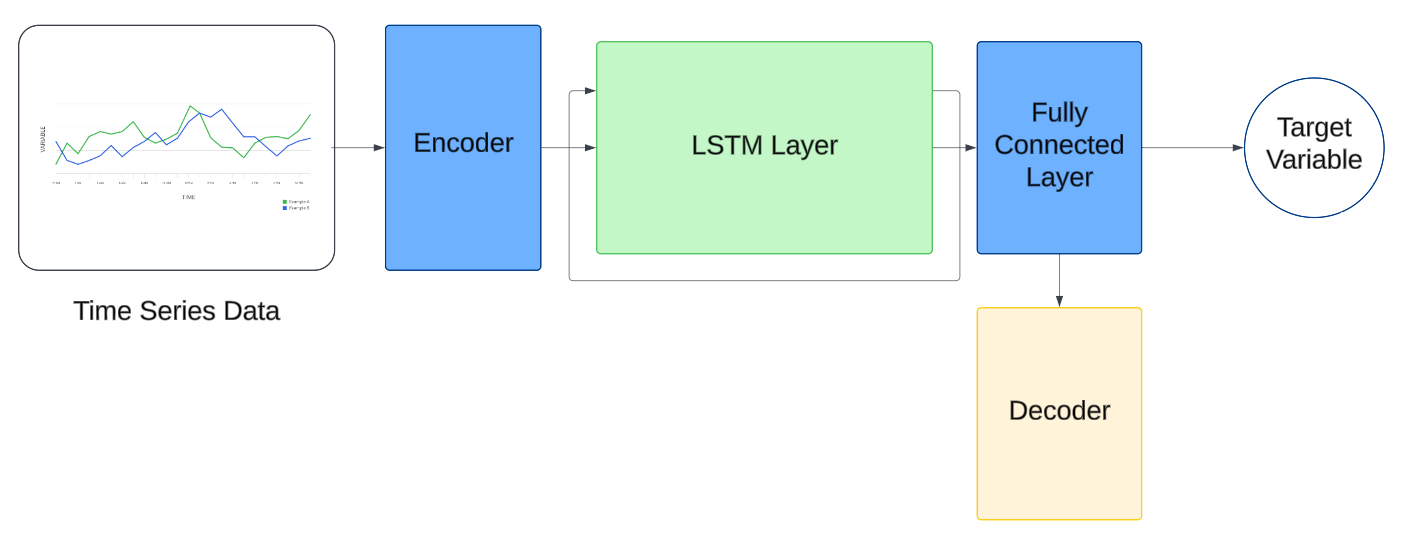
\includegraphics[width=0.8\textwidth]{images/architecture.png}
    \caption{Hybrid Autoencoder-LSTM Model Architecture}
    \label{fig:architecture}
\end{figure}

\begin{itemize}
    \item \textbf{Encoder Layer:} Reduces the input dimensionality by compressing the features into a latent space representation, retaining only the most informative features. This helps eliminate redundant and less relevant information while mitigating the risk of overfitting.
    \item \textbf{Decoder Layer:} Optionally reconstructs the original input from the latent space, enabling auxiliary supervision during training. This reconstruction step ensures the encoder captures the essential structure of the input data.
\end{itemize}

By using an autoencoder, the model focuses on the core features that influence house prices, reducing noise and improving computational efficiency.

\subsection{Time-Series Nature of Data and the Role of LSTMs}

The dataset is inherently sequential, as it includes daily observations of economic indicators. Predicting house prices depends not only on the current values of these indicators but also on their historical patterns and trends. Long Short-Term Memory (LSTM) networks are ideal for such tasks because they:

\begin{itemize}
    \item \textbf{Capture Temporal Dependencies:} LSTMs use gates to selectively remember or forget information from previous time steps, making them effective in identifying trends and temporal relationships in the data.
    \item \textbf{Avoid Vanishing Gradients:} Unlike traditional RNNs, LSTMs are designed to retain information over long sequences without suffering from vanishing gradient issues, enabling them to model long-term dependencies effectively.
\end{itemize}

In this architecture, the compressed latent representation from the autoencoder is fed into the LSTM layers. This combination ensures that the model operates efficiently in high-dimensional spaces while accurately capturing the sequential nature of the data.

\subsection{Advantages of Combining Autoencoders and LSTMs}

The hybrid Autoencoder-LSTM architecture leverages the strengths of both components:

\begin{itemize}
    \item The autoencoder ensures dimensionality reduction, noise elimination, and focus on core patterns, which is essential given the high-dimensional input data.
    \item The LSTM effectively models the temporal dependencies in the reduced feature space, improving the model’s ability to predict trends over time.
\end{itemize}

The combination reduces computational complexity and enhances the robustness and accuracy of predictions by tackling both high-dimensionality and sequential modeling challenges.
    \section{Methodology}

The methodology for predicting house prices involves the integration of data preprocessing, feature engineering, and model training. This section outlines the steps followed to build and evaluate the predictive model.

\subsection{Data Preparation}
The dataset is compiled from three primary sources: MLS Home Price Index (HPI), Consumer Price Index (CPI), and Canada Prime Rate. These indicators, recorded at different frequencies, are unified through resampling and interpolation to ensure consistency:
\begin{itemize}
    \item Monthly CPI data is interpolated to a daily frequency.
    \item Prime rate data, initially provided at discrete time points, is also resampled to daily intervals.
    \item HPI data, sourced from multiple regional Excel sheets, is interpolated for missing values and merged into a single dataset.
\end{itemize}

\subsection{Feature Engineering}
To prepare the data for modeling:
\begin{itemize}
    \item \textbf{Dimensionality Reduction:} Highly correlated features (with a correlation coefficient $>$ 0.6) relative to the target variable, the Single-Family HPI, are removed to avoid multicollinearity.
    \item \textbf{Normalization:} Standard scaling is applied to all features, ensuring zero mean and unit variance for improved model convergence.
    \item \textbf{Dataset Splits:} The data is divided into training (70\%), validation (10\%), and testing (20\%) sets to ensure robust model evaluation.
\end{itemize}

\subsection{Model Training}
The training process involves:
\begin{itemize}
    \item \textbf{Loss Function:} A weighted combination of Mean Squared Error (MSE) for prediction and reconstruction loss for auxiliary supervision ensures the model learns to accurately predict while preserving key data patterns.
    \item \textbf{Optimizer:} The Adam optimizer is used with gradient clipping to stabilize training and prevent exploding gradients.
    \item \textbf{Hyperparameters:} Model parameters, such as the learning rate, number of LSTM layers, and latent space dimensions, are fine-tuned to optimize performance.
\end{itemize}

\subsection{Evaluation Metrics}
The model is evaluated using:
\begin{itemize}
    \item \textbf{Mean Squared Error (MSE):} Quantifies prediction accuracy by measuring the average squared difference between actual and predicted values.
    \item \textbf{R² Score:} Assesses the proportion of variance in the target variable explained by the model.
\end{itemize}

\subsection{Implementation and Logging}
The model is implemented in PyTorch, with:
\begin{itemize}
    \item \textbf{Data Loaders:} Efficiently handling the training, validation, and test datasets.
    \item \textbf{MLflow Integration:} Logging model parameters, training losses, validation scores, and final test results to ensure reproducibility and facilitate future experimentation.
    
    \item \textbf{Visualization:} Key training metrics and model performance are visualized using Matplotlib and logged with MLflow for easy tracking and comparison.
    
    \begin{figure}[H]
        \centering
        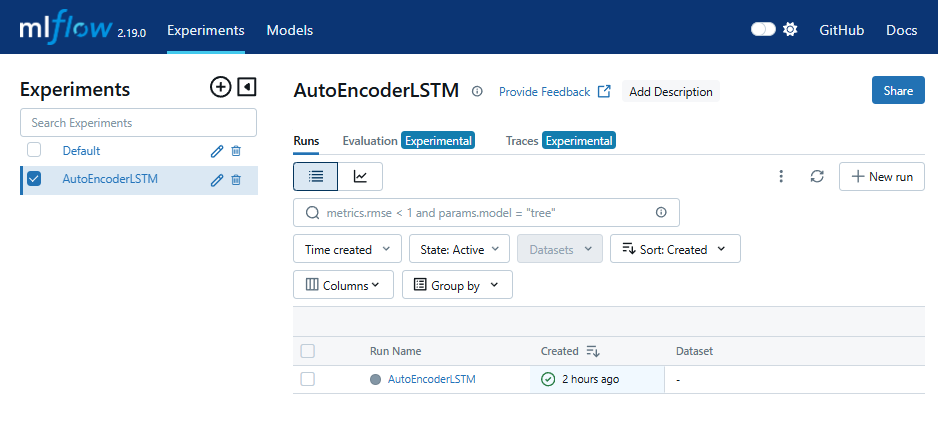
\includegraphics[width=0.8\textwidth]{images/mlflow.png}
        \caption{MLflow logging and visualization of model training metrics.}
        \label{fig:mlflow}
    \end{figure}
\end{itemize}
\subsection{Folder Structure Overview}
The folder structure for the project is organized to ensure clarity, modularity, and ease of maintenance. Below is a detailed explanation of each directory and its contents:

\begin{itemize}
    \item \textbf{.conda Directory:} This directory contains configuration files and dependencies managed by the Conda environment. It ensures reproducibility of the Python environment used for the project.
    
    \item \textbf{data Directory:} This folder contains all the raw datasets required for the project:
    \begin{itemize}
        \item \texttt{CPI\_MONTHLY.csv}: Contains Consumer Price Index (CPI) data, which measures inflation trends.
        \item \texttt{house\_price\_index.xlsx}: Contains MLS Home Price Index (HPI) data for different regions in Canada.
        \item \texttt{Prime-Rate-History.csv}: Includes historical data on Canada's prime interest \\rates.
    \end{itemize}
    Additionally, a subfolder named \texttt{dataloader} is used to store pickled versions of preprocessed data loaders, facilitating quick access to training, validation, and testing datasets.
    
    \item \textbf{mlartifacts and mlruns Directories:} These directories are part of the MLflow tracking system. They store logged model artifacts, parameters, metrics, and experiment run details. MLflow ensures reproducibility and traceability of the model development process.
    
    \item \textbf{model Directory:} This directory contains all files related to the definition and training of the Autoencoder-LSTM model:
    \begin{itemize}
        \item \texttt{\_\_init\_\_.py}: Initializes the model module.
        \item \texttt{model.py}: Defines the architecture of the Autoencoder-LSTM model.
        \item \texttt{params.json}: Stores hyperparameters such as input dimensions, learning rates, and the number of LSTM layers.
        \item \texttt{utils.py}: Includes helper functions for training and evaluation of the model.
    \end{itemize}
    
    \item \textbf{preprocessing Directory:} This directory houses the preprocessing scripts:
    \begin{itemize}
        \item \texttt{load\_cpi.py}: Processes the CPI data, including interpolation and merging of historical revisions.
        \item \texttt{load\_hpi.py}: Handles the HPI data by reading multiple Excel sheets, performing linear interpolation, and merging them into a single dataset.
        \item \texttt{load\_rate.py}: Prepares the prime rate data by resampling and interpolating missing values.
        \item \texttt{\_\_init\_\_.py}: Initializes the preprocessing module.
    \end{itemize}
    
    \item \textbf{report Directory:} This directory is used to store the project's documentation, including the final report and visualizations generated during the project.
\end{itemize}

\textbf{Root-Level Files}
\begin{itemize}
    \item \texttt{main.py}: The main script orchestrates the entire workflow, including data preprocessing, model training, and evaluation. It integrates modules from the preprocessing and model directories.
    \item \texttt{requirements.yml}: Specifies the dependencies and environment configurations required to replicate the project.
    \item \texttt{.gitignore}: Lists files and folders to be excluded from version control.
\end{itemize}

By combining careful data preparation, feature engineering, and the hybrid Autoencoder-LSTM model, this methodology achieves robust and accurate predictions of house prices, addressing both the high dimensionality and sequential characteristics of the dataset.
    \section{Results}

\subsection{Model Parameters and Metrics Analysis}

The Autoencoder-LSTM model was trained using a well-defined set of parameters and evaluated with comprehensive metrics. Below is an in-depth analysis of the results:

\subsubsection{Model Parameters}

\begin{itemize}
    \item \textbf{Cityname:} The model was trained to predict house prices for the city of Regina, focusing on regional trends and characteristics specific to this city.
    \item \textbf{Encoded Dimension (encoded\_dim):} The latent space of the autoencoder compresses the input features into 64 dimensions. This dimensionality is sufficient to capture essential patterns while reducing computational complexity.
    \item \textbf{Input Dimension (input\_dim):} The input data consists of 64 features after preprocessing, indicating the high-dimensional nature of the dataset.
    \item \textbf{Learning Rate:} The learning rate was set to 0.001, providing a balance between fast convergence and stable learning, as evidenced by the smooth decline in training and validation loss.
    \item \textbf{LSTM Hidden Dimension (lstm\_hidden\_dim):} The LSTM network utilized 128 hidden units, enabling it to capture temporal dependencies and long-term trends in the data effectively.
    \item \textbf{Number of LSTM Layers (lstm\_num\_layers):} The model employed a 2-layer LSTM architecture to balance model complexity and computational efficiency.
    \item \textbf{Number of Epochs (num\_epochs):} The model was trained for 50 epochs, sufficient for convergence without overfitting, as demonstrated by the stable loss metrics.
    \item \textbf{Output Dimension (output\_dim):} The output dimension was set to 1, as the task involves predicting a single target variable, the house price index.
\end{itemize}

\subsubsection{Model Metrics}

\begin{figure}[H]
    \centering
    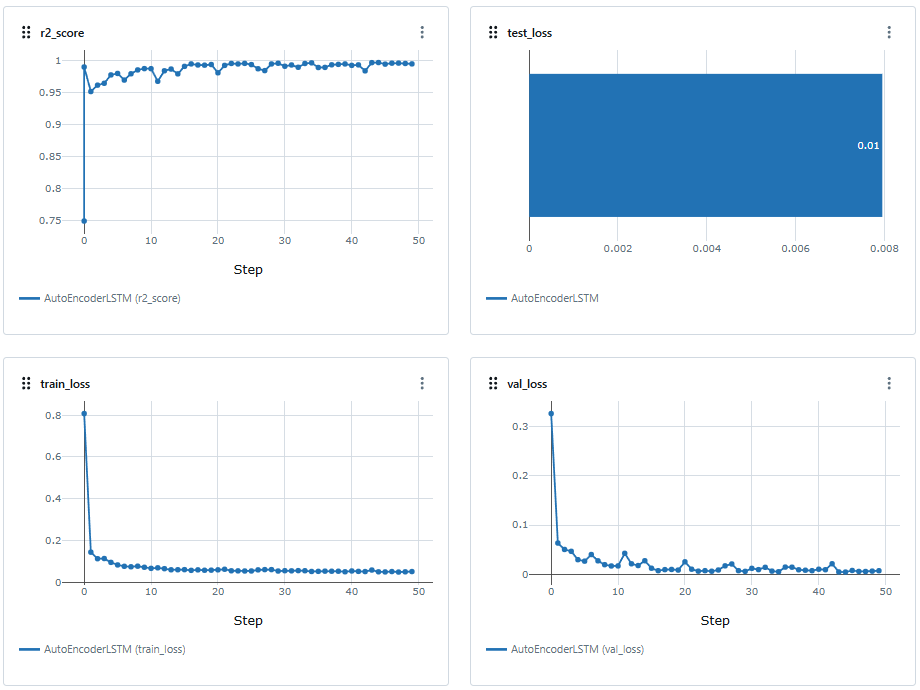
\includegraphics[width=0.8\textwidth]{images/results.png}
    \caption{Model performance metrics visualization.}
    \label{fig:results}
\end{figure}

\begin{itemize}
    \item \textbf{R² Score:} The model achieved an R² score of 0.994, indicating that it explains 99.4\% of the variance in the target variable. This high score highlights the model's ability to accurately predict house prices.
    \item \textbf{Test Loss (test\_loss):} The test loss was recorded as 0.00796, showcasing the model's strong generalization performance on unseen data.
    \item \textbf{Training Loss (train\_loss):} The final training loss was 0.0511, indicating that the model effectively minimized errors during training.
    \item \textbf{Validation Loss (val\_loss):} The validation loss stabilized at 0.00743, closely matching the test loss. This consistency reflects the model's robustness and absence of overfitting.
\end{itemize}

\subsection{Observations and Insights}

\begin{itemize}
    \item \textbf{Strong Generalization:} The close alignment of training, validation, and test losses demonstrates that the model generalizes well to unseen data. This indicates a good balance between underfitting and overfitting.
    \item \textbf{High Predictive Power:} The R² score close to 1 confirms that the model effectively captures patterns in the data and provides highly accurate predictions.
    \item \textbf{Efficiency of Hybrid Architecture:} The combination of autoencoders for dimensionality reduction and LSTMs for sequential modeling contributed to the model's strong performance. The autoencoder reduced noise and redundancy, while the LSTM layers captured temporal dependencies.
\end{itemize}

Overall, this project aims to leverage state-of-the-art machine learning techniques to predict house prices accurately, thereby empowering stakeholders with actionable insights and facilitating informed decision-making in the real estate sector. By addressing the challenges of house price prediction through advanced deep learning models, we aim to contribute to the advancement of real estate analytics and market intelligence.
    \section{Code Implementation}
You can find the code here:
\url{https://github.com/kapeesh-kaul/house-price-prediction}
    \section{Conclusion}
This project successfully developed a robust predictive model for house prices using a hybrid Autoencoder-LSTM architecture. The model effectively addressed the challenges posed by the high dimensionality and sequential nature of the dataset. Key accomplishments include:

\begin{itemize}
    \item \textbf{High Predictive Accuracy:} The model achieved an R² score of 0.994, demonstrating its ability to explain nearly all variance in house prices.
    \item \textbf{Efficient Dimensionality Reduction:} The autoencoder compressed high-dimensional data into a latent space while retaining essential patterns, reducing noise and improving computational efficiency.
    \item \textbf{Temporal Dependency Modeling:} The LSTM layers captured long-term dependencies in the data, enabling accurate time-series predictions.
    \item \textbf{Generalization:} The model exhibited consistent performance across training, validation, and testing datasets, showcasing its robustness and adaptability.
\end{itemize}

These results highlight the effectiveness of combining autoencoders and LSTMs for predictive modeling in complex datasets such as those involving real estate markets. The insights provided by this model can assist stakeholders, including buyers, sellers, and policymakers, in making informed decisions.

\section{Future Work}
While the model demonstrates strong performance, there are opportunities for further enhancements:

\begin{itemize}
    \item \textbf{Scalability Across Regions:} Extend the model to predict house prices for multiple cities or regions, testing its adaptability to different market conditions and demographic trends.
    \item \textbf{Inclusion of Additional Features:} Incorporate external factors such as employment rates, population growth, or geographic attributes to improve the model's comprehensiveness and accuracy.
    \item \textbf{Advanced Hyperparameter Tuning:} Conduct extensive hyperparameter optimization using techniques like grid search or Bayesian optimization to further refine model parameters.
    \item \textbf{Incorporating Seasonal Trends:} Integrate seasonal and cyclical patterns explicitly into the model to capture housing market dynamics better.
    \item \textbf{Real-Time Deployment:} Deploy the model as a real-time prediction tool, allowing stakeholders to access up-to-date house price forecasts through an interactive application or API.
    \item \textbf{Alternative Architectures:} Explore advanced architectures such as Transformer-based models to improve sequential modeling and capture complex relationships more effectively.
    \item \textbf{Explainability:} Enhance model explainability by integrating techniques such as SHAP or LIME to provide insights into feature importance and model decisions.
\end{itemize}

By addressing these areas, the model can be expanded to serve broader applications in real estate analytics and decision-making, enabling more informed and data-driven strategies for various stakeholders.

    \begin{thebibliography}{}

\bibitem{bengio1994}
Bengio, Y., Simard, P., \& Frasconi, P. (1994). Learning long-term dependencies with gradient descent is difficult. \textit{IEEE Transactions on Neural Networks}, 5(2), 157-166.


\bibitem{hochreiter1997}
Hochreiter, S., \& Schmidhuber, J. (1997). Long Short-Term Memory. \textit{Neural Computation}, 9(8), 1735-1780.


\bibitem{hinton2006}
Hinton, G. E., \& Salakhutdinov, R. R. (2006). Reducing the dimensionality of data with neural networks. \textit{Science}, 313(5786), 504–507.

\bibitem{kingma2014}
Kingma, D. P., \& Ba, J. (2014). Adam: A method for stochastic optimization. \textit{arXiv preprint arXiv:1412.6980}.


\bibitem{crea}
Canadian Real Estate Association. MLS Home Price Index (HPI). 


\bibitem{boc}
Bank of Canada. Consumer Price Index (CPI) and Prime Rate History.

\end{thebibliography}


\end{document}